\section{Technical Background}
\label{sec:state:technical}
This chapter give us an overview of important mechanisms used by modern CPUs.
While there are other widely used architectures, such as ARM on mobile devices,
we explore these features in the example of the x86\_64 architecture. \\

I decided to do so because our proof of concept implementation targets the
x86\_64 architecture. Moreover, behavior and implementations of similar concepts
can differ between \gls{isa} and even implementations of the
same \gls{isa} on the microarchitectural plane. I, therefore, note
differences in implementations of x86\_64 whenever appropriate.

\subsection{Operation Modes}
\label{sec:state:technical:modes}
The x86 architecture is rooted in the Intel 8086, designed in 1978. As a 16-bit
microprocessor design, the Intel 8086 physically can only address 64 KiB of
memory. To overcome this limitation, Intel introduced a segmentation-based
addressing mode that, together with the 20-bit address bus, allowed the CPU to
address slightly more than 1 MiB of main memory. Intel 8086 missed features such
as memory protection, code privileges, and multitasking. These features were
important to allow advanced operating systems. These features extended the
instruction set and microarchitecture implemented by the Intel 80286. The Intel
80286 could address, for example, 16 MiB of physical memory through 24 address
bus bits and could address 1 GiB of virtual memory. Moreover, segment registers
now contain an index in a data structure called \gls{gdt}. The \gls{gdt} contains descriptors that store
information on segments, such as base address and access rights. The Intel 80286
implements access rights as rings, and the lower the numerical access level, the
higher the privileges of the executing software are. The introduction of the
\gls{gdt} allowed virtual memory implementation with memory protection. A
new \gls{mmu}, added for the first time on chip in the
80286 allowed fast virtual to physical address translation. \\

When using the features newly added to the 80286 the processor was incompatible
with the original Intel 8086. Because the result would have been that all
software already existing for the Intel 8086 would have been to at least be
recompiled to run on the Intel 80286, Intel designed the new features as an
extension to the older 8086. Deactivating these new features allowed the Intel
80286 to run programs written for the 8086. For this, Intel introduced two
operation modes in the 80286. The operation mode offering compatibility was
called \gls{g_rmode} because the address calculation in the 8086 always
yielded real physical addresses. Because the new 80286 offered memory
protection, the mode was called \gls{g_pmode}. To maintain compatibility
with the Intel 8086, the 80286 first boots in \gls{g_rmode}, as all successors of
the 80286 do. On startup, the code for entering other operation modes must,
therefore, reside in the first MiB of memory. \\

The successor of the Intel 80286, the Intel 80386 extended the architecture to
32-bit and introduced paging to the architecture, allowing paged virtual memory
(cf. \ref{sec:state:technical:paging}). The registers of the 80386 were also
extended to 32-bit. To differentiate between the registers and their extensions,
they are prefixed with ''E''. For example, the instruction pointer register,
formerly identified by IP, becomes EIP with. The Intel 80386 also added the
\gls{smm}. The \gls{smm} is intended
for firmware to execute special tasks such as energy management or other tasks
executed by the firmware. The \gls{smm} code resides in a specially
protected area of the main memory, referred to as \gls{smram}. \gls{smm}
executes with the highest privileges in x86, which is ring -2. With these
changes, the Intel 80386 formed the base for the architecture today known as x86
or IA-32.\\

Successors of the 80386 added support for optional floating point units and
\gls{simd} extensions to the architecture but left the fundamental
\gls{isa} unchanged. It was not until the year 2000 that AMD released its
extensions of the x86 architecture to 64 bit that introduced a new processor
operation mode called \gls{g_lmode} and two sub modes called
Compatibility Mode and 64-Bit mode. This extension by AMD to
the x86 \gls{isa} was first called AMD64 and later largely adopted by
Intel as Intel 64. Today it is also known by the name x86\_64. Compatibility
mode allows the execution of legacy 32-bit and 16-bit code. 64-bit mode extends
the \gls{isa} by 64-bit operands and addresses, and extends all general
purpose registers to 64-bit. Moreover, the 64-bit mode adds eight additional
general-purpose registers and allows instruction pointer relative addressing.
x86 allowed the latter only in control transfer instructions. x86\_64 implements
floating-point arithmetic through the mandatory SSE2 \gls{simd} extension
that was introduced to x86 in 2000 with the Intel Pentium 4 processor. The
number of SSE2 registers is doubled compared to the number in the original x86
extension. Moreover, to allow differentiating between x86 and x86\_64 registers,
AMD added the REX prefix to the specification. As a result, general purpose
registers are prefixed with the letter ''R''. For example, the instruction
pointer registers of x86 (IP) becomes RIP. The number of page table levels to
translate virtual to physical addresses was increased from two to at least
four.\\

Unless otherwise stated, all references I make to \gls{g_lmode} in the remaining
parts of this thesis mean the combination of both sub-modes and therefore the
whole extension implemented by x86\_64.

\subsection{Interrupts and Exceptions}
\label{sec:state:technical:interrupts}
Interrupts and Exceptions are used to call system-specific functions and respond
to special conditions in the CPU or system. Exceptions are raised by the CPU
upon executing software or detecting hardware errors. Interrupts, on the other
hand, are either the result of software interrupt instructions or signals
generated by external hardware, such as keyboard input. Exceptions can be
divided into three types:
\begin{enumerate}
    \item Faults: Result of an error with the instruction to execute
    \item Traps: Result of breakpoint and software interrupt instructions
    \item Aborts
\end{enumerate}
Interrupts, on the other hand, can be divided into two classes:
\begin{enumerate}
    \item Maskable Interrupts: Can be masked. Masking an interrupt means that
          software can temporarily disable them. The interrupt controller holds
          them back until interrupts are enabled again.
    \item \Gls{nmi}~(\gls{nmi}): Software cannot turn off
          \gls{nmi}s. The interrupt controller delivers~
          \gls{nmi}s to the CPU unless it currently serves another~
          \gls{nmi}. When the CPU executes the IRET instruction in the
          interrupt handler, the interrupt controller can deliver the next~
          \gls{nmi}.
\end{enumerate}
The CPU serves exceptions and interrupts by calling the respective interrupt or
exception handler routine. System software can install an interrupt handler by
writing its address into the \gls{idt}. The
\gls{idt} is a data structure containing pointers to interrupt handling
routines. The specification assigns a vector number to each interrupt or
exception. With the help of this vector, the CPU determines what handler to call
by using the interrupt vector as an index in the \gls{idt}. It finds the
\gls{idt} by reading the value of the interrupt descriptor table register
(IDTR). System software is expected to create the \gls{idt} and install
handlers for at least the predefined vectors. Then, the address of the
\gls{idt} is provided by writing to the IDTR before interrupts can be
activated. \\

Over time, interrupt controllers were improved and adapted to new use cases
similar to CPUs. In \gls{g_rmode}, the CPU falls back to using the Intel 8259 or a
compatible programmable interrupt controller, short PIC, that delivers
interrupts to the CPU. Once the PIC delivers an interrupt to the CPU, the CPUs
must serve it and signal the PIC with an \gls{eoi}, that
the serving routine is done, before it can receive the next interrupt. \\

\begin{figure}
    \begin{center}
        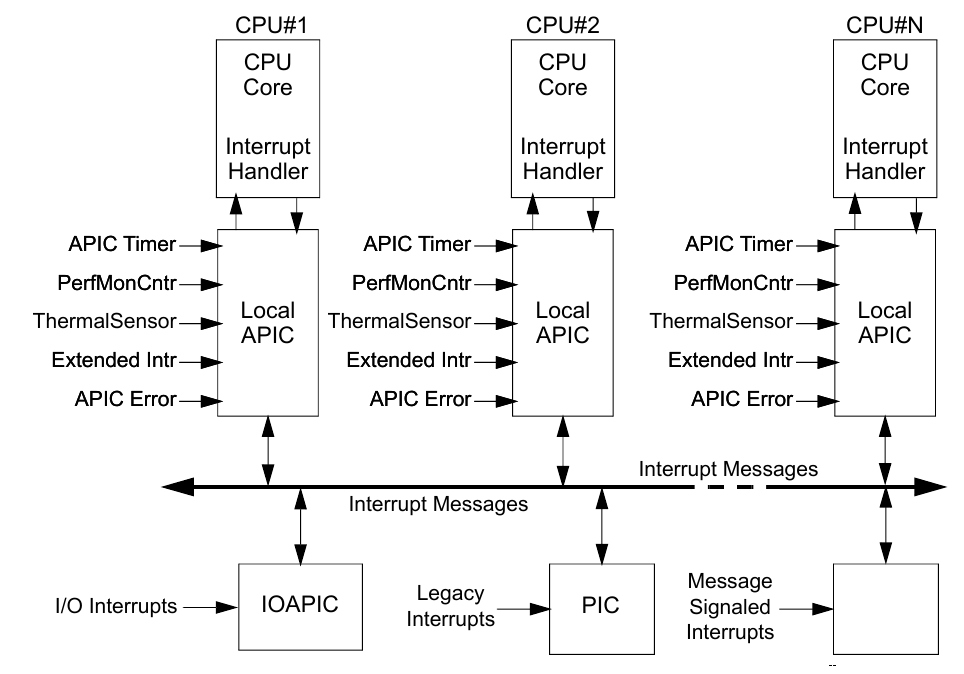
\includegraphics[width=.6\textwidth]{images/lapic_placeholder.png}
        \caption{Illustration of how \gls{lapic}s integrate in a
            multiprocessor system}
        \label{fig:state:technical:lapic}
    \end{center}
\end{figure}
\todo{This is a placeholder}

Intel later introduced the advanced programmable interrupt controller, short
APIC with its 486 processor line to allow the system to operate with multiple
CPUs. In modern CPUs, multiprocessor configurations are prevalent, and each
processor core has its own APIC. Because the APIC is CPU local, these APICs are
called local APICs or \gls{lapic}. \gls{lapic}s
forward interrupts from different sources to the respective CPU core. For
example, the \gls{lapic} receives interrupts such as \gls{ipi}
(\gls{ipi}) from other \gls{lapic}s and legacy interrupts from the
PIC. CPU external devices are deliver their interrupt to the IOAPIC, which
forwards them to the respective LAPIC. Figure~\ref{fig:state:technical:lapic}
shows a schematic view on how the LAPIC of each CPU core integrates into the
system. System software must change the CPU to \gls{g_pmode} to activate the
\gls{lapic} system. After changing to \gls{g_pmode}, system software must
write a valid address to the APIC base address register. All APIC registers are
then mapped to the 4-KiB APIC register space starting at the address specified
in APIC base address register. System software can then access APIC registers
with memory reads and writes to the APIC register space.

\subsection{Caches}
\label{sec:state:technical:caches}
Since 1980, the performance growth of memory and processors has diverged
steadily with an ever-growing gap. Hennessy et al. note a difference in
performance growth of factor 1,000 for a single CPU core and memory
technologies. To highlight the problem, they show the difference between the
peak bandwidth offered by memory and the peak memory bandwidth demand of an
Intel i7 processor of the Nehalem architecture employing four CPU cores. This
processor, which Intel introduced in the year 2009, can generate an instruction
stream that peaks in a maximum bandwidth need of 409.6 GB/sec, while its
dual-channel DDR3 memory interface can yield a maximum bandwidth of 25GB per
second.\cite{hennessy2011computer} With processor implementations growing
further in width, the demand for fast memory further grows. For example, from
November 2023 to January 2024, the number of systems in the TOP500 list that
employed CPUs with 96 cores per socket increased from 0 to 3, with the former
maximum number of cores per socket being 72.\cite{top500} To hide latencies and
bridge the gap between CPU demand and actual main memory bandwidth, CPUs today
employ fast local on-chip memory to buffer data they already accessed. If they
reaccess this memory item, they can use these buffers to speed up access. This
on-chip buffer described is called cache.\\

The cache is an integral component organized in a multi-level hierarchy in
modern CPUs. In this hierarchy, the lowest and the nearest to the core level,
called the L1 cache, implements the fastest access. Most modern x86 CPUs divide
their L1 cache into two parts: L1D for data and L1I instructions. With
increasing levels, caches grow in size but tend to be slower. For example, while
the L1 Cache of Nehalem CPUs offers only one cycle of latency, the L3 Cache of
the same CPU has a latency of 35 cycles.\cite{hennessy2011computer}\\

When the CPU tries to access data, it first queries the fastest cache. If the
CPU can locate the data in the cache, this is called a cache hit. On a cache
hit, the CPU can profit from reduced access time and improved bandwidth. The
opposite of a cache hit is called a cache miss, in which the CPU subsequently
queries the next level in the memory hierarchy. If it finds the data needed, it
loads these into the nearest cache for faster access. Caches can only store a
limited number of items, organized in cache lines. Each cache line is either 32
or 64 bytes in size, with x86\_64 processors mainly implement a cache line size
of 64 bytes. Cache lines are a copy of the main memory, and the processor uses
this copy for all of its operations unless otherwise configured. The processor
loads data in cache line size granularity from the main memory. Modern x86 CPU
designs organize caches in sets. In a set, all of the cache lines are
exclusively mapped to a specific, non-overlapping address range of physical
memory. The number of cache lines a physical address can be mapped to is
indirectly proportional to the number of sets in a cache, which is called the
associativity of the cache. For example, a cache with one cache line per set is
called a direct mapped cache because a physical address can only be mapped to
one set and its cache line. The hardware cost of a mapped cache is the lowest.
Direct-mapped caches bring the drawback of a higher probability of conflict
misses. A conflict miss in caching describes the situation in which the
processor loads data from the main memory and has to evict lines from the cache
because no suitable cache line is available. Because a physical address range
with multiple cache line-sized chunks is exclusively mapped to one line in a
directly mapped cache, loads from the same range can cause conflict misses.
Conversely, in a cache with a single set containing all cache lines, all
physical addresses can be mapped to each line in the set. Such a cache is called
fully associative and has the highest hardware costs but comes with the
advantage of minimal fragmentation. Often, processors implement a trade-off
between hardware cost and flexibility of the cache. Such caches are called
$n$-way set associative, where $n$ is the number of cache lines in each set. On
a cache fill, the processor first finds the set of cache lines to which it can
map the physical address. Once it identifies the set, the processor can place
the data in any line. \\

Caches use the principle of locality, which consists of two kinds of locality.
The first is called spatial locality. Spatial locality describes the observation
that if a program accesses data from the main memory, data located at nearby
addresses will be the target of future accesses with a high probability. In this
case, the CPU tries to guess the size of the loaded structure to load parts
missing in the cache in advance. If the CPU then accesses the neighbor of the
first data, it already resides in the cache, lowering the latency. The second
principle is temporal locality, which states that a program soon reuses memory
references with a high probability. The CPU can, therefore, gain performance by
storing recently used data in the cache for reuse.\\

Modern caches are still small compared to the size of the main memory. For
example, CPUs of the recent AMD Zen 5 microarchitecture have an L1 cache size of
92 KiB (data and instruction combined) and 32 MiB of L3 cache shared between the
cores, from which eight physically exist on the same chiplet. The same CPU
supports 128 GiB of main memory, which is seven orders of magnitude larger than
the L1 and 4 orders of magnitude larger than the L3 cache.\todo{cite amd zen
    five paper (When writing this SLUB Shibboleth was broken...)} Caches, therefore,
can not buffer the content of the whole main memory and need strategies for
their management. For example, CPUs of the Nehalem microarchitecture use a
pseudo least recently used (LRU) strategy to manage their cache's
content.\cite{hennessy2011computer} With this, cache lines are marked as
frequently or less frequently used. The least frequently used lines are evicted
from the cache and replaced by the newly cached data. Evicted lines are moved
one level up in the hierarchy. Other management strategies are the least
frequently used (LFU) or a first-in-first-out (FIFO) policy. Next to eviction
strategies, different strategies for writing data back to main memory exist:
\begin{itemize}
    \item \textbf{write-back}: Data modified in the cache is stored and written
          back to the main memory later. Until cache and main memory are
          synchronized, the region in main memory is marked as dirty through a
          dedicated status bit. Cache coherency protocols are required to allow
          multiple devices to access the same memory range.
    \item \textbf{write-through}: The Changes in the cache are instantly written
          to the main memory. These writes can slow down program execution
          because of costly main memory writes.
    \item \textbf{cache-disable}: The CPU cache is disabled, and the CPU
          performs all memory operations using the main memory.
\end{itemize}
Legacy x86 control cache settings with configuration bits in the control
register CR0. In modern x86\_64 processors, systems software sets the write-back
strategy on page granularity (c.f. Chapter~\ref{sec:state:technical:paging}).
X86\_64 processors ignore the write-through setting and use the page-level
settings instead. \cite{amd_manual} The default in x86\_64 processors ist to use
a write-back strategy. For this, processors implement coherency protocols. A
widely used coherency protocol is called MESI. MESI is an acronym of the four
states "modified," "exclusive," "shared," and "invalid." An extension to MESI is
MOESI protocol, which additionally introduces the "owned" state. The states of a
cache line, as specified by the AMD programmers manual, are:
\begin{itemize}
    \item \textbf{Modified}: The copy in the processor's cache is the most
          recent and modified. The copy in the main memory needs to be updated.
          No other processor in the system maintains a copy.
    \item \textbf{Owned}: Similar to shared state, but copy in main memory can
          be stale. All other processors must hold their copy in the shared
          state.
    \item \textbf{Shared}:  The copy is the most recent and correct copy of the
          data. Other processors may hold copies, too. Main memory holds the
          most recent and correct copy, too, if no processor holds a copy with
          \textbf{Owned} state.
    \item \textbf{Exclusive}: The processors and the main memory's copy are the
          most recent and correct copies. No other processor holds a copy.
    \item \textbf{Invalid}: The local copy is invalid. Either main memory or
          other processors hold a valid copy.
\end{itemize}
\todo{inclusiviy}

An interesting difference in the x86\_64 implementation of Intel and AMD
processors are the cache coherency and inclusion policies. AMD processors use
MOESI as a cache coherency protocol to use, as mentioned
before.\cite{amd_manual} Intel processors, on the other hand, use MESI as a
coherency protocol. \cite{intel_sdm} The use of different coherency protocols to
synchronize data between multiple CPU cores has a direct effect on the
inclusivity of the cache implementation. On all current x86\_64 multicore CPUs,
the \gls{llc} is shared among all cores for synchronization and uses one
of the coherency protocols. CPUs produced by Intel largely use an inclusive
\gls{llc}. An inclusive cache describes a cache containing items in lower
cache levels. If an item is modified in a lower cache level, the changes are
automatically propagated to the higher inclusive cache level. The opposite of an
inclusive cache is an exclusive cache design, as used by most AMD CPUS.
Exclusive caches do not necessarily contain items of lower cache levels, and the
synchronization of modified items needs to be propagated in other ways. The
additional "owned" state of the MOESI protocol solves this issue.

\subsection{Hardware Performance counters}
\label{sec:state:technical:hpc}
The first x86 CPU implementing hardware \gls{pmc} \gls{pmc} and
documenting them was the Intel Pentium Pro in 1995, implementing the P6
microarchitecture.\cite{intel_sdm} The x86\_64 \gls{isa} specificities
four freely programmable architectural hardware
\gls{pmc}s.\cite{amd_manual} Concrete processor implementation can offer
additional counters. Similarly, the \gls{isa} specifies architectural
events that must be present in every processor implementing x86\_64. Additional
events are vendor and implementation-specific. The four counters can be
programmed to count any event supported by the respective processor
implementation. Vendors of x86 CPUs publish what processor supports what
additional events in their manuals. Moreover, a CPU notes what events it
supports in the result of the \gls{g_cpuid} instruction. \\

In x86 hardware, Performance counters are implemented by a set of two \gls{msr}s
(\gls{msr}) per counter. One \gls{msr} can be programmed by system
software with the event to measure, while a second \gls{msr} counts the
occurrence of the respective event. As noted, programming has to be done by
system software with elevated privileges. Reading \gls{pmc}s can be done
with privileged instruction or from user space with the RDPMC instruction. In
this way, a program can poll the values of counters. The system software can
also program a threshold for a \gls{pmi}. Once the
\gls{pmc} values exceed the threshold, the \gls{pmi} is triggered,
offering an alternative to expensive polling techniques.\\

When I use hardware \gls{pmc}, I must use the proper technique adopted to
the environment in which I read the counter values. Das et al. found in a
comprehensive survey that noise from the system is often present, e.g. context
switches influence the values of performance counters. \cite{das_sok_2019}
Moreover, some counter events are over-counted while the CPU can undercount
others.\cite{weaver_non-determinism_2013} It is therefore important to check the
right conditions for using hardware counters and verify that they work
correctly.

\subsection{Paging}
\label{sec:state:technical:paging}
\begin{center}
    \begin{figure}
        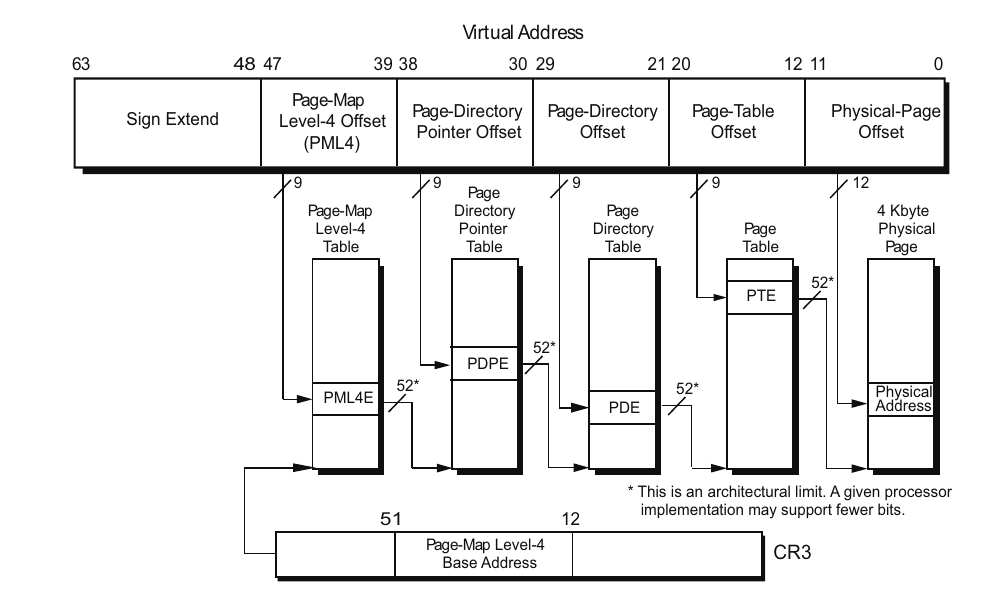
\includegraphics[width=\textwidth]{images/paging_placeholder.png}
        \caption{Illustration of Virtual Address Translation with 4 Levels of Page Tables}
        \label{fig:state:technical:paging}
    \end{figure}
    \todo{This is a placeholder}
\end{center}

Historically, paging replaced segmentation in x86 for working with virtual
memory. Virtual memory is an abstraction that does not allow direct addressing
of physical main memory through programs. Instead, a program sees the whole
address space as available. Once the program tries to allocate memory, system
software creates a virtual memory address and hands it to the program. System
software decides through its mapping implementation, through which physical
memory the respective virtual memory is backed. Virtual memory, therefore,
allows system software to decide if a given virtual address is backed by main
memory or to move it to secondary memory, such as disk storage. Moreover, two or
more virtual addresses can be mapped to the same physical memory, allowing
efficient use of shared program libraries. Mapping happens transparently to the
program, which means that the program does not have to worry about what memory
is used to back its virtual memory physically.\\

Paging is an approach to virtual memory that replaces segment-based virtual
memory in modern x86 CPUs. With paging, the system divides memory into chunks
equal to the page size. System software uses pages to manage memory on
allocation requests from programs. Pages are virtual memory chunks mapped to
page frames in physical memory. Access rights are controlled by system software
that sets the respective rights in the pages and is enforced by hardware with
page granularity. Hardware translates virtual to physical addresses. This
process is called page translation. In the following, we view the paging
implementation of x86\_64 in more detail to explain page translation in more
detail.\\

Hardware uses page tables for page translation that are hierarchically
organized. Each page table forms a level in the table hierarchy and is the size
of one page, storing references (addresses) to the next lower level. The last
page table in this hierarchy stores the address of the physical page frame. By
default, x86\_64 uses pages of size 4 KiB. Because x86\_64 uses 64-bit
addresses, each page table can store 512 entries.
Figure~\ref{fig:state:technical:paging} shows the page translation of a virtual
64-bit address in x86\_64 with a page table hierarchy of four levels and a page
size of 4 KiB. \\

The virtual address is divided into a 12-bit field used as an index in the
physical page and four 9-bit fields, which the hardware uses as an index to
access the content of the respective page level. The remaining address bits are
sign extensions of bit 52, forming a canonical address. The hardware must
perform a page table walk to resolve the virtual address. For the first step of
a page table walk, the processor locates the address of the first page table, in
this case, the PML4 table. The address of the PML4 is written by system software
to CR3 after it creates the page table. In doing so, the system software does
not write the entire 64-bit address to CR3. Instead, it writes the most
significant bits beginning from bit 12 because memory is accessed at page
granularity, meaning the lower 12 bits are irrelevant to addressing the page
frame. Most x86\_64 implementations furthermore only support $2^{52}$ byte of
addressable memory and therefore use 52 bits of the 64-bit address space. This
results in the 40 bits stored in CR3, as seen in
~Figure~\ref{fig:state:technical:paging}. To access PML4, the CPU reconstructs
its address from CR3. It uses the 9-bit index of the PML4 offset field in the
virtual address to find the Page-Map-Level 4 entry containing the address of the
next page table, the Page-Directory-Pointer table. The CPU accesses this table
and all successor tables similarly until it locates the physical page. To access
the data that belongs to the virtual address, the CPU uses the last 12 bits of
the virtual address to locate the data on the physical page. \\

As the page table walk is expensive, the \gls{mmu} automatically stores
the translated addresses in a cache called \gls{tlb}.
Each CPU manages its page tables and \gls{tlb}. System software must
maintain consistency between page tables and each \gls{tlb} by
invalidating individual entries or the entire \gls{tlb}. If system
software invalidates an entry, the CPU has to complete a page walk for this
virtual address, upon which the MMU updates the \gls{tlb}. The INVLPGB
can additionally be used to invalidate a range of TLB entries and broadcast
these invalidations to other CPUs. \\

\begin{figure}
    \begin{center}
        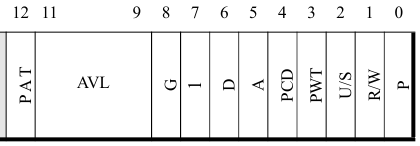
\includegraphics[width=.6\textwidth]{images/paging_rights_placeholder.png}
        \caption{Layout of the lowest 12 bits in a page table entry}
        \label{fig:state:technical:paging_rights}
    \end{center}
\end{figure}
\todo{This is a placeholder}

The unused lower 12 bits of each table entry are used for management properties,
such as access rights management. Figure~\ref{fig:state:technical:paging_rights}
shows the layout of the lower 12 bits of a page table entry. The present bit is
another property stored in the lowest 12 if of a page table's entry. It
indicates if the page the respective entry points to was initialized and loaded
to the page table. If this bit equals 0, the CPU generates a \gls{pf}
(\gls{pf}) exception and expects system software to load the respective
entry. The CPU also generates a \gls{pf} if software violates access
rights. A second bit important for this thesis is the Page-Level Cache Disable
(PCD) bit. If the PCD bit is set, the CPU cannot cache the respective page. Bit
3 (PWT) controls page-level write-through. If system software sets this bit, the
page table has a write-through caching policy.

\todo{write about bootflow}
\subsection{Bootflow of Modern x86 CPUs}
\label{sec:state:technical:boot}
